\section{Target and Detectors}
The COMPASS experiment comprises large number of detectors, for identifying and measuring the particles coming out of interaction vertices. Additionally, There are also detectors which monitor the particle beams and trigger other components to decide when the signals should be read out or not. In this section, the basic functionalities of different kinds of detectors are introduced shortly. 

\begin{figure*}[!ht]
	\centering
	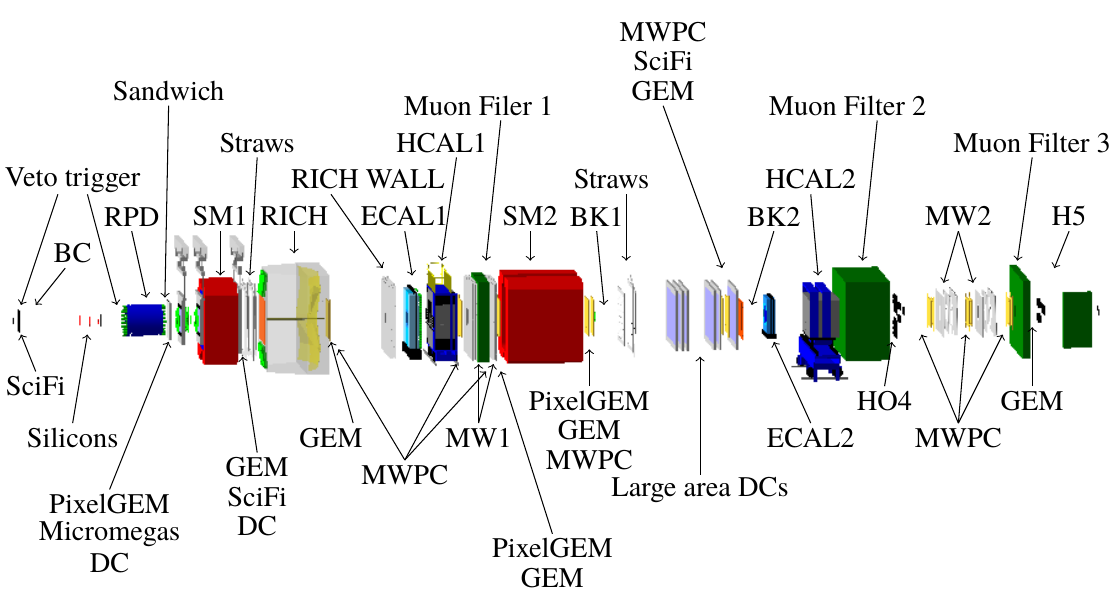
\includegraphics[width=\textwidth]{detector_layout}
	\caption{Layout of the COMPASS experiment. The length of the whole setup is around 50 meters. The beam comes from the left side of detectors and hits the target, which is surrounded by the recoil-proton detector (RPD). On the right-hand side of the target, two different sets of detectors are used to measure out-going particles with small and large scattering angles.\cite{Henri}}
	\label{fig:detec_layout}	
\end{figure*}

\subsection{Particle beam and target}
To create the projectile particle beam, the proton beam, which is accelerated by the Super Proton Synchrotron (SPS), is firstly directed into Beryllium. From the nuclear reaction between proton and Beryllium nucleus, a secondary hadron particle beam is created, which functions as incoming particle beam for the scattering experiment. The beam is composed of $\pi^-$ ($96.8\%$), $K^-$ ($2.4\%$), $\bar{p}$ ($0.8\%$) for the 2008 data under investigation\cite{Henri}. The proton target, onto which the beam is diverted, is in form of liquid hydrogen stored in a \SI{40}{\centi\meter} height cylindrical container. 

\subsection{Detector layout}
\label{subsec:Detector_layout}
\begin{figure}[!th]
	\centering
	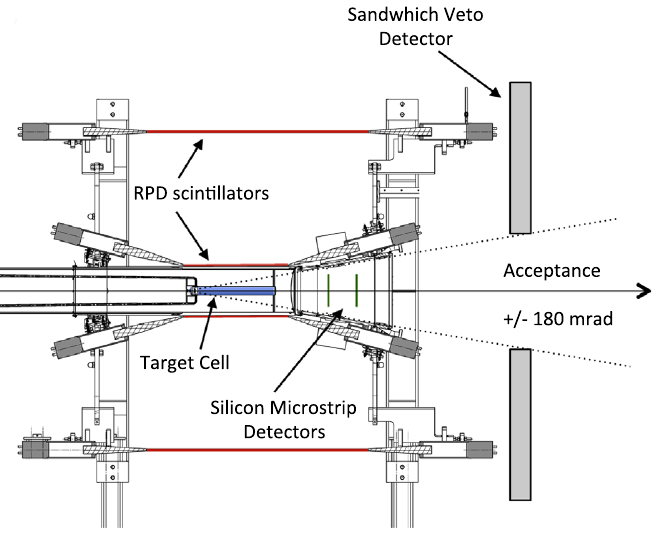
\includegraphics[width=0.5\textwidth]{sandwich}
	\caption{Scheme of the detectors around the target region. The sandwich veto on the right vetos events which include particles emerging from the target with large scattering angles. Source: \cite{sandwich}}
	\label{fig:sandwich}
\end{figure}

The layout of COMPASS experiment is shown in figure \ref{fig:detec_layout}. Proton target is surrounded by the RPD (recoil-proton detector). Upstream of target locate detectors such as SciFi (scintillating fiber), BC (Beam counter) and silicon detectors. The coincidence of signals from SciFi and BC is used for the beam trigger, setting the time reference of whole system. The silicon detectors are applied for determining the location of the projectile beam, which is further used to calculate the position of the primary vertex. Downstream very close to the target, there are sandwich veto and PixelGEM/Micromegas/DC (Pixel GEM detector, micromegas detectors and drift chamber). The function of sandwich veto is to reject the signal readout when the scattering angle of out-going particle is too large to measure. Specifically, scattering angle is the angle between the beam direction and the momentum direction of the outgoing particle. The structure of sandwich veto can be seen in figure \ref{fig:sandwich}, where the veto can be triggered if the scattering angle is out of acceptance range. Behind the sandwich veto, tracking detectors (PixelGEM/Micromegas/DC) are implemented to measure the angles of out-going particles with high accuracy and resolution. Downstream further away from the target, two different sets of detectors are set up for measuring out-going particles with small and large scattering angles. 

The first set, located in the front, is used as large angle spectrometer (LAS). The major components of LAS are SM1 (solenoid magnet 1), tracking detectors, RICH (ring-image Cherenkov detector), ECAL1, HCAL1 and Muon filter. SM1 provides the magnetic field to deviate charged particles. The degree of deviation is measured by the tracking detectors on the both sides, which can calculate the momentum of out-going charged particles. The RICH detector downstream SM1 is used to improve the permanence of experiment by identifying $\pi^-$ from $K^-$ in high intensity environment\cite{RICH}. ECAL1 is an electromagnetic calorimeter used to measure the energy of particles like electrons or photons while HCAL1, a hadron calorimeter, is used to measure the energy of hadrons. Muons can be identified by tracking detectors behind a muon filter, which intercepts all particles except muon. The second set, located at the end of the experiment, is called small angle spectrometer (SAS). Most of its components have the same functionalities as their counterparts in LAS. The main additional detectors in SAS contains two BKs (beam killer), which are basically two scintillating counters. They are used to veto the non-interacting particle beams\cite{sandwich}. Besides the difference in measuring range of scattering angle, another major difference for LAS and SAS is about the structural design: detectors in LAS has holes in the center to allow the outgoing particles with small scattering angle to pass to SAS; On the other hand, detectors in SAS also have  small holes as passages for the non-interactive particle beams. 




